% !TeX spellcheck = en_US
% !TeX encoding = UTF-8
% !TeX root = ../thesis.tex

\chapter{Fundamentals}
This chapter introduces basic concepts used throughout this thesis.
First, we discuss the basics of reinforcement learning and
the problem of robot learning.
Next, we give an overview of policy search,
a sub-field of reinforcement learning,
as one method to solve the robot learning problem.
The Kullback-Leibler divergence (KL) is
introduced as an important information theoretic
measure of similarity metric between probability
distributions \citep{kullback1951information}.
Having discussed the underlying basics, we can then
introduce the MORE algorithm \citep{abdolmaleki2015model}.
Next we will look at filtering from a Bayesian Estimation viewpoint and
review the Kalman filter for parameter estimation. Finally, we
look at some data preprocessing techniques employed.

\section{Reinforcement Learning}
Reinforcement Learning (RL) is a subfield of Machine Learning
concerned with agents
learning to interact with their environment and
solving specific tasks.
This is done through exploration and trial-and-error. The agents
try to discover cause and effect relationships between their actions.
Compared to supervised learning and unsupervised learning it
more closely resembles the way we humans learn by interacting
with our environment. \\
As \citet{sutton2018reinforcement} puts it,
the term reinforcement learning relates to a class of problems,
solution methods and the field that studies these problems and solutions.
Some success stories of RL include mastering the game of Go
\citep{silver2016mastering} and Atari games \citep{mnih2013playing}.
Generally, RL is applicable to a large range of problems.
Whereas in supervised learning the best action is presented to the system,
the agent in a reinforcement learning setting receives a
reward (or punishment) for each action.
To gain information about the rewards the agent needs
to explore previously unused actions.
The decision of daring to try new things or to keep performing safe
well-known actions is known as the
\textit{exploration-exploitation tradeoff}.
In general, the agent should exploit known actions that
give decent reward, but he first
has to try different things to learn about these actions,
and then he has to progressively focus in on them.
The reward signal is typically a single scalar value,
hence the amount of information
the agent receives is minimal compared to
supervised and unsupervised learning approaches.

The classical approach to formalizing problems in RL is through
Markov Decision Processes (MDPs).
MDPs are a mathematical
framework for decision making in deterministic and stochastic environments.
MDPs focus on only three aspects
- sensation, action and goal, which are central
for reinforcement learning problems.
MDPs satisfy the Markov property, which
states that ``the future is independent
of the past given the present''. In our case, this means
the next state $s'$ and the reward
only depend on the previous state $s$ and
action $a$ \citep{sutton1992reinforcement}.
An MDP can be formally defined as a tuple $(S, A, P, r)$:

\begin{itemize}
\item a set of states $s \in S$ that describe the environment,
\item a set of actions $a \in A$ that can be performed by the agent in
  the environment
\item a transition function $P(s_{t+1} |\, s_t, a_t)$ that
  gives the probability of a new
  state $s_{t+1}$ after an action $a_t$ has been taken in state $s_t$,
\item and a reward function $r(s_t, a_t)$ that specifies
  the immediate reward after taking action
  $a_t$ in state $s_t$.
\end{itemize}

The Markov property can be expressed as
$$ P(s_{t+1} |\, s_t, a_t, s_{t-1}, a_{t-1}\dots) = P(s_{t+1} |\, s_t, a_t). $$
This recapitulates the notion of state - a state is a sufficient statistic
for predicting the future, rendering previous observations irrelevant.
In robotics, we may only find some approximate notion of state.

We model the agent and its environment as a state $s \in S$.
The agent may perform action $ a \in A$ which can be
either discrete or continuous.
For every action step, the agent receives a reward $R$,
which is a scalar value.
The overarching goal is to find a mapping from states to actions,
called policy $\pi$, that picks actions in a way that
the reward is maximized.
We can distinguish an \textit{episodic} setting
from an on-going task.
In the episodic setting
the task is restarted after
the end of an episode and the goal is
to maximize the total reward per episode.
In on-going tasks the goal
is to simply achieve high average reward over
the whole life-time or one can use a formulation
with a discounted return (weighting the
future and past differently).

Generally, the goal is to find an optimal policy $\pi^*$,
a mapping from states to actions that
maximizes the expected return $J$.
Optimal behavior can be modeled in
different ways, resulting in different
definitions for expected return:
\begin{itemize}
\item for a finite-horizon model with horizon $H$ we get
$$ J = E \left\{\sum^H_{t=0} R_t \right\}, $$

\item a discounted reward can be modeled with
  a discount factor $\gamma$ (with $0 \leq \gamma < 1)$, which yields
$$ J = E \left\{\sum^{\infty}_{t=0} \gamma^{\; t} R_t \right\}. $$
\end{itemize}

Reinforcement learning can also be seen as
general case of optimal control as in \citet{sutton1992reinforcement}.
While optimal control assumes perfect knowledge, RL uses approximations
and data-driven techniques.

%TODO: - write about Value learning, and shortly name traditional methods (multiarmbandit,
%DP, Temporal difference learning)


\section{Robot Learning}
The sub-field where reinforcement learning and machine learning
intersect with robotics is called \textit{Robot Learning}. It aims to bridge
the gap between programmed robots,
with fine tuned controllers  and fully autonomous robots.
As proposed in \citet{deisenroth2013survey}, robot control can be modeled as
a reinforcement learning problem. \\
The state space $\mathbf{x}$ in robotic tasks is high dimensional and
made up of
the internal state of the robot (e.g., joint position, body position,
camera images)
and external state (e.g. object locations, lighting). The true state is
not observable and also not noise free. 
The robot chooses its next motor control $u$ according to a policy $\pi$.
This policy $\pi$ may
be deterministic $u = \pi(x)$ or stochastic $u \sim \pi(x,u) = P(u |\,x)$.
The motor command $u$ alters the state according to the probabilistic
transition function $p(\mathbf{x}_{t+1} |\, x_t, u_t)$.
This transition function
is not known, in model-based policy search this
function is learned from data and
used to improve the policy.
Collectively, the states and actions of the robot form a
trajectory $\tau = (x_0, u_0, x_1, u_1,...)$ which is also called
a rollout or a path.
There has to be a numeric scoring system assessing the quality
of the robots trajectory and returning a reward signal $R(\tau)$.
For episodic learning tasks, the task ends after a given number $T$ time
steps. Then, the accumulated reward $R(\tau)$ for a trajectory is given by

$$ R(\tau) = r_T(x_T) + \sum^{T-1}_{t=0} r_t(x_t,u_t) $$

where $r_t$ is an instantaneous reward function
(e.g. a punishment for energy consumed)
and $r_T$ the final reward. When performing a reaching task this may take the
form of a quadratic punishment term for deviation from the goal posture.

If we consider an infinite-horizon for an on-going task we get
$$ R(\tau) = \sum^{\infty}_{t=0} \gamma^{\; t} r(x_t, u_t) $$
where $\gamma \in [0,1)$ is a discount factor that discounts
rewards further in the future.

Many tasks in robotics can thus be formulated as choosing an optimal control
policy $\pi^*$ that maximizes the expected accumulated reward
$$ J_{\pi} = \mathbb{E}[R(\tau) |\, \pi] = \int R(\tau) p_{\pi}(\tau) d\tau $$
where $R(\tau)$ defines the objectives of the task, and $p_{\pi}(\tau)$ the
distribution over trajectories $\tau$.

Formulating robotic tasks in this way allows us to apply methods from
reinforcement learning to them. 

\subsection{Challenges}
Except for simple tabular problems reinforcement
learning can generally be considered a difficult problem.
One reason for this is that the reward signal may be given
only occasionally and
even then it may be unclear which of
the agents actions were responsible for a certain
reward signal. 

Robotics is different compared to other fields where reinforcement learning
is used. First of all, the states and actions of the robots in the
real world are inherently continuous requiring us to
deal with the resolution into a discrete representation.
In addition, the state space can have a high dimensionality and
working with real world systems on real hardware is costly and
makes manual interventions necessary.
Robots require algorithms to run in real-time and working with
real sensors further introduces discrepancy between sensing and
execution.
Generally, the state represented by sensors slightly lags behind the real
state due to processing and communication delays. This is in stark contrast to
most other reinforcement learning algorithms, which assume actions to
take effect instantaneously.


Most traditional methods from RL like
TD-learning \citep{sutton2018reinforcement}
have been unfit for these particular requirements of robotic tasks.
Stressing the importance of robotics as a special testing ground for RL that
demands new developments and innovative research.
We will now discuss some problems encountered when applying
RL to robotics. This treatment focuses only on a certain
set of challenges and is not meant to be exhaustive.

\subsubsection{Curse of Dimensionality}
The term ``Curse of Dimensionality'' was coined by \citet{Bellman:1957} when
he explored optimal control in higher dimensions and encountered
an exponential explosion of the states and actions.
For example, in our evaluation we run a simulation of a
simple planar reaching task
with a 5 link robot arm using Dynamic Movement Primitives \citep{ijspeert2002learning}
for policy representation and get a 25 dimensional state.
Especially modern anthropomorphic robots tend to have many degrees of
freedom, which further increases the dimensionality.

The agent in RL generally needs to collect data throughout the entire
state-space to ensure global optimization. In robotics the agent
often has to deal with high dimensional states and actions
due to many degrees of freedom which makes this global optimization
in many cases infeasible.
To alleviate this problem  a widespread idea is to use expert demonstration
to get a good initialization for the agent's policy. This
eliminates the need to explore the entire search space, instead the
agent can focus on locally optimizing the initial policy.
This concept of imitation learning focuses on the problem of ``learning
from demonstrations'' which plays an important role
for robotics \citep{Osaetal18}. Imitation learning
will enable domain experts to teach motions and
skills without special knowledge about robotics, which will be crucial
when robots start making their way from factories into everyday life.

\subsubsection{Curse of Real-world Samples}
Robot hardware is expensive and suffers from wear and tear, making
costly maintenance necessary. Hence, safe methods for real robots
should avoid big jumps in policy updates, as such sudden changes may
result in unpredictable movements and consequently damage the robot.
This constraint is commonly referred to as \textit{safe exploration}.
Whereas in traditional reinforcement learning
safe exploration does not receive much attention,
it has become a key issue for robot learning \citep{schneider1997exploiting}.

When working with a real physical robot,
different external factors like temperature may change the robot's
dynamics and
additionally uncertainty from the sensors makes it difficult to reproduce and
compare results.

Most tasks also require a ``human in the loop'' who either
supervises the robot
or resets the setup after one episode. Even if this step
can be automated the data generation is very slow
compared to other applications of RL which are based only on simulation.
For a single robot the training time has a natural limit
and in total only relatively few executions can be completed.
One method for gathering more data is ``collective robot learning''
described in
\citet{kehoe2015survey}. The idea is for multiple robots to
share their data on trajectories, policies and outcomes.
Currently, this seems only
viable for large corporations with significant capital and therefore
stresses the importance of developing sample efficient algorithms.
Thus, in robot learning the constraint of using only a small number of trials
is given more weight than limiting memory consumption or
computational complexity.


\subsubsection{Curse of Goal Specification}
Defining a good reward function in robot reinforcement learning is
difficult and often needs a lot of domain knowledge and expertise.
There are certain trade-offs to keep in mind, for example performing
a powerful swing for a hitting task may yield high reward but may damage
or shorten the life-time of the robot.
Further, reinforcement learning algorithms may solve tasks
in unintended ways by exploiting the reward function in an unforeseen fashion
\citep{ng1999policy}.
An alternative to specifying the reward function manually
is Inverse Reinforcement Learning \citep{russell1998learning}
The goal of inverse reinforcement learning is to recover the unknown
reward function from the expert's trajectories.


$$~$$
The discussed challenges illustrate the difficulty of the optimal control
problem in robotics.
Generally, autonomous learning algorithms are rarely employed on robots
for real daily usage. Also, most
algorithms are over fitted to a particular robot architecture
and do not generalize to other robots easily.
Even minor flaws or errors in the employed method can completely prevent
success of learning.
Nonetheless, appropriately chosen algorithms and rewards functions
can already achieve promising results \citep{kober2013reinforcement}, but as 
a large number of different methods exist 
there is no clear general recipe for robot learning,
underlining the fact that robot learning still has a lot of open problems,
and will continue to grow as a research field.

\subsection{Policy Search}
Many traditional methods in RL try to estimate the
expected long-term reward of a policy for each state $\mathbf{x}$
and time step $t$, which leads to formulation of the value
function $V^{\pi}_t(\mathbf{x})$.
With the value function we can asses the quality of executing action
$\mathbf{u}$ in state $\mathbf{x}$. This assessment is used
to directly compute the policy by action selection or to update
the policy $\pi$. As value function methods typically require
to fill the complete action-space they struggle with
the high dimensionality encountered in robotics.
Thus, policy search methods have become more common
for applying RL to robotics.
Policy search methods opposed to value-based methods
use parameterized policies $\pi_{\theta}$ to search
directly in the parameter space $\Theta$
of the policies $(\text{with }\theta \in \Theta)$. This allows using RL with
high-dimensional continuous action spaces encountered
in robotics by reducing the search space of possible policies.
Policy search further allows the usage of predefined
task-appropriate policy representations like Dynamic
Movement Primitives \citep{schaal2005learning}, as well
as easily integrating imitation learning
for policy initialization.

Generally, we can divide policy search into model-free and model-based and
differentiate whether stochastic or deterministic trajectories are used.
Model-free policy search uses trajectories from the robot directly
for updating the policy. Model-based methods use the data
from the robot to first learn a model of the robot. This model is then used
to generate trajectories that are used for policy updates.
Due to their simplicity and by avoiding the need of learning a model,
which further introduces the problem of under-modeling,
model-free methods have been employed to a wide range of problems
\citep{deisenroth2013survey}.

The most important concept in policy search is computing the policy updates.
Both model-free and model-based policy search methods use policy
gradients (PG) which employ gradient ascent for maximizing
the expected return.
The REINFORCE algorithm introduced in \citet{williams1992simple}
is an example for a model-free method using policy gradients.
The PILCO (probabilistic inference for learning control)
policy search framework \citep{deisenroth2011pilco}
is an example for a model-based approach.
Another way to compute the policy updates 
is using the Expectation-Maximization algorithm \citep{bishop2006pattern},
by formulating policy
search as an inference problem. One model-free method for this category
is the Policy learning by Weighting Exploration with the Returns (PoWER)
algorithm \citep{kober2011policy}.
The third category of policy updates we look at
are information-theoretic (Inf. Th.) approaches
based on the Kullback-Leibler Divergence (\Cref{sec:kl}).
The relative entropy policy search algorithm (REPS)
\citep{peters2010relative}
and the MORE algorithm (\Cref{sec:more}) fit into this category.
In \Cref{fig:policy}
we give a graphical overview of the different policy search methods.

$~$
\begin{figure}[ht!]
  \centering
  \scalebox{0.9}{
\usetikzlibrary {backgrounds,fit}
    \begin{tikzpicture}
      \draw (1, 0.5) node [draw=black, rounded corners] (data) {Policy Search};

      \draw (-2.4, -1) node [fill=blue!80!black!30, rounded corners](model_free) {Model-free};
      \draw [-] (data) -- (model_free);      
      \draw (-2.4, -2) node [fill=red!80!black!30, rounded corners](free) {Stoch. Traj.};
      \draw [-] (model_free) -- (free);      
      \draw (-3.5, -3) node [fill=green!80!black!20, rounded corners](free_pg) {PG};
      \draw (-2.5, -3) node [fill=green!80!black!20, rounded corners](free_em) {EM};
      \draw (-1.25, -3) node [fill=green!80!black!20, rounded corners](free_inf) {Inf. Th.};
      \draw [-] (free) -- (free_pg);
      \draw [-] (free) -- (free_em);
      \draw [-] (free) -- (free_inf);
      
      
      \draw (4, -1) node [fill=blue!80!black!30, rounded corners] (model) {Model-based};
      \draw [-] (data) -- (model);
      
      \draw (2.25, -2) node [fill=red!80!black!30, rounded corners] (model_stoch) {Stoch. Traj.};
      \draw [-] (model) -- (model_stoch);      
      \draw (1.25, -3) node [fill=green!80!black!20, rounded corners](stoch_pg) {PG};
      \draw (2.25, -3) node [fill=green!80!black!20, rounded corners](stoch_em) {EM};
      \draw (3.5, -3) node [fill=green!80!black!20, rounded corners](stoch_inf) {Inf. Th.};
      \draw [-] (model_stoch) -- (stoch_pg);
      \draw [-] (model_stoch) -- (stoch_em);
      \draw [-] (model_stoch) -- (stoch_inf);

      
      \draw (6, -2) node [fill=red!80!black!30, rounded corners] (model_det) {Det. Traj.};
      \draw [-] (model) -- (model_det);      
      \draw (5, -3) node [fill=green!80!black!20, rounded corners](det_pg) {PG};
      \draw (6, -3) node [fill=green!80!black!20, rounded corners](det_em) {EM};
      \draw (7.25, -3) node [fill=green!80!black!20, rounded corners](det_inf) {Inf. Th.};
      \draw [-] (model_det) -- (det_pg);
      \draw [-] (model_det) -- (det_em);
      \draw [-] (model_det) -- (det_inf);

      %%%%%%%%%%%%%%%%%%%%%%%%%%%%%%%%%%%%%%%%%%%%%%%%%%%%%%%%%%%%%%
      % Examples
      %%%%%%%%%%%%%%%%%%%%%%%%%%%%%%%%%%%%%%%%%%%%%%%%%%%%%%%%%%%%%%
      \draw (-4.75, -5) node (examples) {\small \textbf{Examples:}};      
      \draw (-3.25, -5.6) node (reinforce) {REINFORCE};
      \draw (-1.25, -5.2) node (power) {PoWER};
      \draw (0.6, -5.4) node (reps) {REPS};
      \draw (2.2, -5.1) node (more) {MORE};      
      \draw [thick, dotted] (free_pg) to[out=-90,in=90] (reinforce);
      \draw [thick, dotted] (free_em) to[out=-90,in=90] (power);
      \draw [thick, dotted] (free_inf) to[out=-90,in=90] (reps);
      \draw [thick, dotted] (free_inf) to[out=-75,in=90] (more);      

      
      % \draw (4, -5.75) node (pegasus) {PEGASUS};
      \draw (5.5, -5) node (pilco)
      {$~~~~~~~~\quad\quad\quad\quad\quad$ PILCO $~~~~~~~\quad\quad\quad\quad\quad$};
      \draw [thick, dotted] (det_pg) to[out=-90,in=90] (pilco);

      \begin{scope}[on background layer]
        \node [thick, dashed, draw=black, rounded corners, fill=black!5,fit=
        (model_free) (free) (free_pg) (free_em) (free_inf)]{};
      \end{scope}
      
      \begin{scope}[on background layer]
        \node [thick, dashed, draw=black, rounded corners, fill=black!5,fit=
        (model) (model_det) (model_stoch)
        (det_pg) (det_em) (det_inf)
        (stoch_pg) (stoch_em) (stoch_inf)]{};
      \end{scope}
      
      \begin{scope}[on background layer]
        \node [thick, draw=black,fit=
        (examples)
        (reinforce) (power)
        (reps) (pilco)]{};
      \end{scope}
    \end{tikzpicture}
}
    \caption{\small
      Categorization of policy search into model-free
      and model-based with differentiation
      based on trajectory generation and policy update methods.
      For model-free methods stochastic trajectory (Stoch. Traj.) generation
      directly samples the trajectories from the robot
      and in the model-based case from the learned model of the robot.
      Some model-based methods also use deterministic trajectory
      (Det. Traj.) prediction where the goal is to 
      analytically predict the trajectory distribution
      instead of sampling from the system. 
      The drawing is based on
      \citet{deisenroth2013survey}.
    }
    \label{fig:policy}
\end{figure}

% - TODO: include figure for policy search taxonomy
% (recreated from \citet{deisenroth2013survey})
% also include examples for each type (REINFORCE, REPS, PILCO,...)


In this thesis, we will focus on model free policy search methods
where the trajectories are generated by ``sampling'' from
the robot and information theoretic policy updates are used.
More specifically we will formulate our approach
in the setting of stochastic
search algorithms, which are general black-box optimizers.
They are applied in a wide range of fields like operations research and
machine learning.
Since these algorithms do not use any knowledge about the
objective function it is straightforward to
apply them to policy search in the episode-based formulation.

Using stochastic search algorithms we keep an upper-level policy
$\pi_{\omega}(\theta)$ which selects the parameters of the
actual control policy $\pi_{\theta}(\mathbf{u} |\, \mathbf{x})$ of the robot.
Instead of directly finding the parameters $\theta$ of the
lower-level policy we want to find the parameter vector $\omega$ which
defines a search distribution over $\theta$. We can then use this
search distribution to directly explore the parameter space.


\section{Kullback-Leibler (KL) Divergence}
\label{sec:kl}
Several algorithms that can be used for model-free policy search like
NES \citep{wierstra2014natural} and
REPS \citep{peters2010relative} 
rely on the Kullback-Leibler divergence, also
known as the relative entropy, for controlling
the difference between the old and updated policy.
Working with real robots additionally requires to perform safe exploration.
Big exploration steps may result in damaging the hardware.
Specifically, it measures the Shannon entropy of one distribution
relative to the other.
The KL divergence from $q$ to $p$ is defined as
$$ \text{KL}(p || q)
= \int p(\theta) \text{ log} \left(\frac{p(\theta)}{q(\theta)}\right)
d \theta $$
where $p$ and $q$ are continuous probability distributions.
Note, that in general the relative entropy is not symmetric under interchange
of the distributions $p$ and $q$.
% In general $KL(p || q) \neq KL(q || p) $, therefore
% in a mathematical sense it is not strictly a distance.

%%%%%%%%%%%%%%%%%%%%%%%%%%%%%%%%%%%%%%%%%%%%%%%%%%%%%%%%%%%%%%%%%%%%%%%%%%%%%%%%
%\section{Constraint Optimization}
%- look at mechano informatik slides
%
%In constraint optimization we want to maximize a function subject to constraints on
%the variables. Generally we have the following problem formulation
%
%\begin{align}
%  \min_{x\in \mathbf{R}^N} f(x)  \text{subject to}
%  \begin{cases}
%    c_i(x) = 0 \\
%    c_i(x) \geq 0
%  \end{cases}
%\end{align}
%
%
%Introducing the Lagragian function we get
%\begin{align}
% \mathcal{L}(\pi, \eta, \omega) = 
%\int \pi(\theta) \mathbf{R}_{\theta} d\theta \; + \; 
%\eta  \left(\epsilon - \int \pi(\theta) \text{ log}
% \frac{\pi(\theta)}{q(\theta)} d\theta\right)
% - \; \omega \left(\beta + \int \pi(\theta) \text{ log}(\pi(\theta)) d\theta\right)
%\end{align}
%
%We can now construct an alternative problem the dual function, which is easier to
%solve than the primal problem. We optimize for the Lagragian multipliers.
%
%%%%%%%%%%%%%%%%%%%%%%%%%%%%%%%%%%%%%%%%%%%%%%%%%%%%%%%%%%%%%%%%%%%%%%%%%%%%%%%%

\section{MORE Algorithm}
\label{sec:more}
Model-Based Relative Entropy Stochastic Search
(MORE) \citep{abdolmaleki2015model} is a
stochastic search algorithm that can be used
as a policy search method for episodic reinforcement
learning tasks. The key idea is
using information-theoretic policy updates
by bounding the relative entropy (Kullback Leibler divergence)
between two subsequent policies.
As MORE uses no gradient information and requires only function evaluations
of the objective function it can be seen as
a type of stochastic search algorithm and can be used
for black box optimization problems.
The essential difference of MORE compared to previous algorithms using
the KL-bound like REPS \citep{peters2010relative} lies in utilizing
a quadratic surrogate model of the objective function
to  satisfy the KL-bound in closed form without approximations.
On top of that it
introduces a lower bound constraint on the entropy of the new distribution
to avoid premature convergence.

The MORE algorithm can be used to maximize an objective function
$f(\mathbf{x}): \mathbb{R}^n \rightarrow \mathbb{R}$. The goal is
to find one or more parameter vectors $\mathbf{x} \in \mathbb{R}^n$ with the
highest possible objective value. For this the algorithm maintains
a search distribution over $\mathbf{x}$ for which the
expectation over the reward is maximized. To accomplish this, the
MORE algorithm iteratively draws samples from the search
distribution, implemented
as a multivariate Gaussian distribution, i.e.
$\pi(\mathbf{x}) = \mathbf{N}(\mathbf{x} |\, \mu, \Sigma)$.
This distribution corresponds to an upper-level policy
and is parameterized by the mean and covariance matrix.
In each iteration, $N$ samples are drawn from the
search distribution. Each sample $\mathbf{x}$ is then
evaluated on the objective function yielding the corresponding
objective value $r$, this constitutes the data
$\{\mathbf{x}^{\;k}, r^{\;k}\}_{k=1...N}$ which is
used to compute a new search distribution.
This iterative process is run until the algorithm converges.

% TODO: 3 pictures on sphere function
% 1. MORE sampling from search distrib
% 2. resulting surrogate model
% 3. updated search distribution

\subsection{MORE Framework}
To satisfy the bound on the relative entropy between subsequent
search distributions and the bound on the entropy while
optimizing the objective function
we use the theory of constraint optimization \citep{boyd2004convex}.
In constraint optimization we want to maximize a function
$f(x)$ under a set of equality constraints and inequality constraints.
\begin{equation}
  \label{eq:constraint}
  \begin{aligned}
    \text{maximize } \quad f(x)& \\
    \text{subject to } \quad g_i(x)& = 0, \quad i = 1, \dots, m\\
    c_j(x)& \leq 0, \quad j = 1, \dots, p
  \end{aligned}                       
\end{equation}

With this we can now formulate the constraint optimization
problem to obtain a new search
distribution that maximizes the expected objective value
while upper-bounding the KL-divergence and lower-bounding the entropy
of the search distribution at the same time
\begin{equation*}
  \begin{aligned}
    \max_{\pi} \quad &\int \pi(\mathbf{x}) f(\mathbf{x}) d\mathbf{x}, \\
    \text{subject to } \quad &\text{KL }(\pi(\mathbf{x})||q(\mathbf{x}))
    \leq \epsilon, \\
     &H(\pi) \geq \beta, \\
     &1 = \int \pi(\mathbf{x}) d\mathbf{x},
  \end{aligned}
\end{equation*}
where $H(\pi) = - \int \pi(\mathbf{x}) \log \pi(\mathbf{x}) d\mathbf{x}$
denotes the entropy of the search distribution.
The parameters $\epsilon$ and $\beta$ are hyperparameters to control the
exploration-exploitation trade-off.
The $\epsilon$ can be chosen freely to control the step size of the
policy update. Generally, its size will depend on the specific problem
and the amount of available samples.
The bound $\beta$ is defined such that the relative difference
between the entropy
of the policy $H(\pi)$ and a minimum exploration policy $H(\pi_0)$ is
decreased
for a certain percentage:
$$ H(\pi) - H(\pi_0) \geq \gamma (H(q) - H(\pi_0))
\rightarrow \beta = \gamma (H(q) - H(\pi_0) + H(\pi_0) $$
The key idea of the MORE algorithm is to use a surrogate model
of the objective function
for satisfying the bound on the KL-divergence.
The surrogate model has the following form
\begin{align*}
  % TODO: explain why using 1/2 or not?
  f(\mathbf{x}) \approx \hat{f}(\mathbf{x}) =
  %-\frac{1}{2}
  \mathbf{x}^T \mathbf{R} \mathbf{x}
  + \mathbf{x}^T \mathbf{r} + r.
\end{align*}
A quadratic model is sufficient, since the exponent
of a Gaussian distribution
is also quadratic and thus it would not be possible to exploit
the additional information of a more complex surrogate model.
For estimating the surrogate model the original approach of
MORE employs a Bayesian dimensionality
reduction method and linear regression. 

% With the assumption of $\pi$ being Gaussian we
% get the solution \Cref{policy_update}
% for updating the mean and covariance matrix
% of the search distribution.

By using the theory of Lagrange multipliers and duality \citep{boyd2004convex}
we obtain the solution to the constraint optimization problem 
(for details see \Cref{more_appendix}).
Assuming $\pi$ to be Gaussian, solving the dual problems yields

\begin{equation}
  \label{policy_update}
  \begin{aligned}
    \pi_{t+1} &= \text{N}(\mu_{t+1}, \Sigma_{t+1}) \\
    \mu_{t+1} &= (\eta \Sigma_{t}^{-1}\mu_t + \mathbf{r}) / (\eta + \omega) \\
    \Sigma_{t+1} &= (\eta \Sigma_t^{-1} + \mathbf{R}) / (\eta + \omega),
  \end{aligned}
\end{equation}

where $\eta$ and $\omega$ are the Lagrangian multipliers obtained
by minimizing
the corresponding dual function. In addition,
the linear term  $\mathbf{r} \in \mathbb{R}^n$ and
the quadratic term $\mathbf{R} \in \mathbb{R}^{n\times n}$  of
the current surrogate model are
used to update the policy.
With these equations, we can iteratively update the search distribution.


\section{Bayesian Filtering}
Optimal filtering is concerned with estimating the state
of a time-varying system
which is indirectly observed through noisy measurements.
This section will focus on optimal filtering from a Bayesian perspective
and is largely based on \citet{sarkka2013bayesian}.

The term ``Bayesian'' refers to inference methods that represent
``degrees of certainty'' using probability theory. They are fundamentally
based on applying
Bayes' rule to update the degree of certainty given data.
More generally, as \citet{gelman2013bayesian} puts its, Bayesian inference
is the process of fitting a probability model
to a set of data and summarizing the result by a probability distribution
on the parameters of the model and on unobserved quantities such
as predictions for new observations.

Filtering methods are widely used in robotics
to deal with noisy sensor measurements. This
includes tasks like object tracking, robot control and
robot localization \citep{chen2011kalman}.
Since robots need to make decisions based on relatively small amounts
of data, it is common to adopt a Bayesian perspective when
using filtering methods and for 
reasoning about the environment in general \citep{thrun2002probabilistic}.

\subsection{Bayesian Parameter Estimation}
In general, when using Bayesian models for estimating
\textit{unknown parameters} $\theta$, the following probability distributions
are used:

\begin{itemize}
\item \textbf{Prior Distribution:}
Encodes the information on parameter $\theta$ before seeing any
observations. When we are uncertain about our prior information
we can choose a high variance of the distribution or use a
non-informative prior (which imposes the minimal amount of structure
on the data).
$$ p(\theta) = \text{information on parameter } \theta
\text{ before seeing any observations} $$

\item \textbf{Measurement Model:}
Models the relationship between true parameters and the measurements.
$$ p(y |\, \theta) = \text{distribution of observation } y
\text{ given the parameters } \theta $$

\item \textbf{Posterior Distribution:}
The conditional distribution of the parameters given the observations.
It represents the updated belief about the parameters
after obtaining the measurements. It can be computed by using Bayes' rule.
$$ p(\theta |\, y) = \frac{p(y |\, \theta) p(\theta)}{p(y)}
\propto p(y |\, \theta) p(\theta) $$
\end{itemize}

\subsection{Optimal Filtering as Bayesian Inference}
The goal of optimal filtering can be seen as solving a statistical
inversion problem where
the unknown quantity is a potentially vector valued
time series $\{\mathbf{x}_0, \mathbf{x}_1, \mathbf{x}_2,...\}$ which
is observed through a set of noisy measurements
$\{\mathbf{y}_1, \mathbf{y}_2,...\}$, as depicted in \Cref{fig:inversion}.

\begin{figure}[ht!]
    \centering
    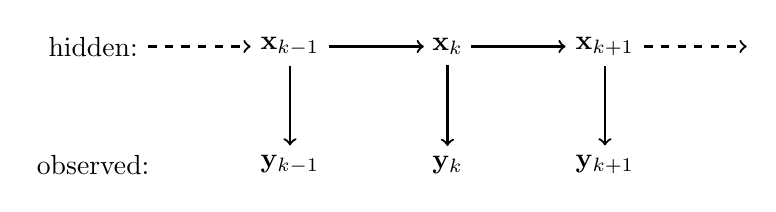
\begin{tikzpicture}
      \draw (0, 0) node {hidden:};
      \draw [->][dashed, thick] (0.7, 0) -- (2, 0);
      \draw (2.5, 0) node (x1) {$\mathbf{x}_{k-1}$};
      \draw [->][thick] (3, 0) -- (4.2, 0);
      \draw (4.5, 0) node (x2) {$\mathbf{x}_k$};
      \draw [->][thick] (4.8, 0) -- (6, 0);
      \draw (6.5, 0) node (x3) {$\mathbf{x}_{k+1}$};
      \draw [->][dashed, thick] (7, 0) -- (8.3, 0);

      \draw (0, -1.5) node {observed:};

      \draw (2.5, -1.5) node (y1) {$\mathbf{y}_{k-1}$};
      \draw [->][thick] (x1) -- (y1);
      \draw (4.5, -1.5) node (y2) {$\mathbf{y}_k$};
      \draw [->][thick] (x2) -- (y2);
      \draw (6.5, -1.5) node (y3) {$\mathbf{y}_{k+1}$};
      \draw [->][thick] (x3) -- (y3);
    \end{tikzpicture}
 \caption{A sequence of  hidden states $\mathbf{x}_k$ is indirectly
 observed through noisy measurements. Drawing recreated from \citep{sarkka2013bayesian}.}
    \label{fig:inversion}
\end{figure}

% TODO: reproduce figure of hidden variables and observations
% in Tikz side by side
% with  simple signal example  and measurement

We want to estimate the hidden states from the observed
measurements. Solving this problem in a Bayesian
sense means we 
need to compute the joint posterior distribution of all
states given all the measurements, for this we can
use Bayes' rule.
This yields a batch solution to the statistical estimation problem
resulting in the equation
\begin{equation}
  \label{eq:bayes}
  p(\mathbf{x}_{0:T} |\, y_{1:T})
  = \frac{p(y_{1:T} |\, \mathbf{x}_{0:T}) p(\mathbf{x}_{0:T})}
  {p(y_{1:T})}
\end{equation}
where $p(\mathbf{x}_{0:T})$ is the prior distribution defined by the dynamic
model, $p(y_{1:T} |\, \mathbf{x}_{0:T})$ is the likelihood model for the
measurements and $p(y_{1:T})$ is the normalization constant defined as
$$ p(y_{1:T}) = \int p(y_{1:T} |\, \mathbf{x}_{0:T})
p(\mathbf{x}_{0:T}) d \mathbf{x}_{0:T}.$$
This formulation is unfit for dynamic estimation tasks where
we receive measurements one at a time, since
at each time step we would have to
recompute the full posterior distribution. As the number of
time steps increases, also the dimensionality of the full posterior
would increase making computations intractable.
If we instead only compute selected marginal distributions we can
make computation feasible again. For this we need to restrict
our dynamic models to probabilistic Markov sequences, with a
transition probability distribution $p(\mathbf{x}_k |\, \mathbf{x}_{k-1})$
that depends only on the previous state.


In \textit{Bayesian filtering and smoothing} the following marginal
distributions are of interest

\begin{itemize}
\item \textbf{Filtering distributions} computed by the
  Bayesian filter are the marginal distributions of the
  current state $\mathbf{x}_k$ given the current and previous measurements
  $y_{1:k} = \{y_1,...,y_k\}$
  $$ p(\mathbf{x}_k |\, y_{1:k}), \quad k = 1,...,T.$$
\item \textbf{Prediction distributions} which can be computed with
  the prediction step of the Bayesian filter are the marginal
  distributions of the future state $\mathbf{x}_{k+n}$, with $n$ steps
  after the current time step
  $$ p(\mathbf{x}_{k+n} |\, y_{1:k}), \quad k = 1,...,T \;\;\; n = 1,2,...$$
\item \textbf{Smoothing distributions} computed by the Bayesian smoother
  are the marginal distributions of the state $\mathbf{x}_k$ given
  a certain interval $y_{1:T} = \{y_1,...,y_T\}$ of measurements with
  $T > k$
  $$ p(\mathbf{x}_k |\, y_{1:T}), \quad k = 1,...,T$$
\end{itemize}

% maybe add illustration with bars from särkkä book

We will focus on the filtering distribution,
as we use it for our surrogate model estimation problem.

For the filtering distribution we can formulate the recursive Bayesian
solution to the statistical inversion problem as follows:
\begin{enumerate}
\item The distribution of measurements is modeled by the likelihood
  function $p(y_k |\, \mathbf{x}_k)$ and the measurements are assumed
  to be conditionally independent
\item In the beginning at time step zero all information about $\mathbf{x}$
  is contained in the prior distribution $p(\mathbf{x}_0)$
\item The measurements are assumed to be obtained one at a time,
  first $y_1$ then $y_2$ and so on. The key idea is to use the posterior
  distribution from the previous time step as the current prior
  distribution
  \begin{align*}
    p(\mathbf{x}_1 |\, y_{1})
    &= \frac{1}{Z_1} p(y_1 |\, \mathbf{x}_1) p(\mathbf{x}_0), \\
    p(\mathbf{x}_2 |\, y_{1:2})
    &= \frac{1}{Z_2} p(y_2 |\, \mathbf{x}_2) p(\mathbf{x}_1 |\, y_1), \\
                            &\vdots \\
    p(\mathbf{x}_k |\, y_{1:k})
    &= \frac{1}{Z_k} p(y_k |\, \mathbf{x}_k) p(\mathbf{x}_k |\, y_{1:k-1}), \\
                            &\vdots \\
    p(\mathbf{x}_T |\, y_{1:T})
    &= \frac{1}{Z_T} p(y_T |\, \mathbf{x}_T) p(\mathbf{x}_{T-1} |\, y_{1:T-1}),
  \end{align*}
  with the normalization term $Z_k = \int p(y_k |\, \mathbf{x}_k)
  p(\mathbf{x}_k |\, y_{1:k-1})
  d \mathbf{x}_k$. 
\end{enumerate}

This recursive formulation of Bayesian estimation has several useful
properties. First of all it can be considered as the
\textit{online learning} solution to the Bayesian learning problem.
As each step in the recursive estimation is a full Bayesian update step,
batch Bayesian inference is a special case of recursive Bayesian
inference. Due to the sequential nature of the estimation we can model
what happens to the unknown quantity $\mathbf{x}$. This turns out
to be the basis of filtering theory, where time behavior is modeled
by assuming the quantity to be a time-dependent stochastic process
$\mathbf{x}(t)$.

\subsection{Least Squares}
To ease the application of Bayesian filtering to our specific problem
at a later stage we will now discuss a simple regression problem.
First we are going to derive the least squares solution, as
we use a least squares (LS) approach for comparison in our experiments.

We consider a simple linear regression problem,
\begin{equation}
  \label{regression_problem}
  y_k = x_1 + x_2 \, t_k + \epsilon_k
\end{equation}
where we assume that the measurement noise is zero mean Gaussian with
a given variance $\epsilon_k \sim \mathcal{N}(0, \sigma^2)$ and that the
prior distribution of the
parameters $\mathbf{x} = (x_{1} \; x_{2})^T$ is
Gaussian with known mean and covariance
$\mathbf{x} \sim \mathcal{N}(\mathbf{m}_0, \mathbf{P}_0)$. Note that
in this section the parameters $\mathbf{x}$ are assumed to stay constant.
We now want to estimate
the parameters $\mathbf{x}$ from a set of measurement
data $\mathcal{D} = \{(t_1, y_1),...,(t_T, y_T)\}$.

In compact probabilistic notation the linear regression model
can be written as
\begin{equation}
  \label{regression_model_1}
  \begin{aligned}
    p(y_k |\, \mathbf{x}) &= \mathcal{N}(y_k |\, \mathbf{H}_k \, \mathbf{x}, \sigma^2) \\
    p(\mathbf{x}) &= \mathcal{N}(\mathbf{x} \, |\,
    \mathbf{m}_0, \mathbf{P}_0)
  \end{aligned}
\end{equation}
Here $\mathbf{H}_k = (1 \;t_k)$ is the design matrix and
contains the regressors and $\mathcal{N}(\cdot)$ denotes
the Gaussian probability density
function (see \Cref{gauss_pdf}). The row vector $\mathbf{H}_k$ is denoted
in matrix notation, to avoid using different notation for scalar
and vector measurements.
The batch solution can then be easily obtained by application of Bayes'rule
$$ p(\mathbf{x} | \, y_{1:T})
\propto p(\mathbf{x}) \prod^T_{k=1} p (y_k | \, \mathbf{x}) $$
$$ = \mathcal{N}(\mathbf{x} | \, \mathbf{m}_0, \mathbf{P}_0)
\prod^T_{k=1} \mathcal{N}(y_k |\, \textbf{H}_k \mathbf{x}, \sigma^2). $$

Because the prior and likelihood are Gaussian, the posterior distribution
in turn is also Gaussian and denoted by
$$ p(\mathbf{x} | y_{1:T}) = \mathcal{N}(\mathbf{x} | \,
\mathbf{m}_t, \mathbf{P}_t). $$

By completing the quadratic form in the exponent
we get the equations (\ref{LS}) for the mean and covariance
of the posterior distribution.
%- TODO: Do calculation in Appendix, (use canonical form)

\begin{equation}
  \label{LS}
  \begin{aligned}
    \mathbf{m}_T &= \left[ \mathbf{P}^{-1}_0 + \frac{1}{\sigma^2} \mathbf{H}^T \mathbf{H}
                   \right]^{-1} \left[\frac{1}{\sigma^2} \mathbf{H}^T \mathbf{y} +
                   \mathbf{P}^{-1}_0 \mathbf{m}_0 \right] \\
    \mathbf{P}_T &= \left[\mathbf{P}_0^{-1} + \frac{1}{\sigma^2} \mathbf{H}^T \mathbf{H}
                 \right]^{-1}
  \end{aligned}
\end{equation}
where $\mathbf{H}_k = (1 \;t_k)$ and
$$ \mathbf{H} =
\begin{pmatrix} \mathbf{H}_1 \\ \vdots \\ \mathbf{H}_T \end{pmatrix}
= \begin{pmatrix}
  1 \quad t_1 \\
  \vdots \quad \vdots \\
  1 \quad t_t
\end{pmatrix},
\quad \quad y = \begin{pmatrix} y_1 \\ \vdots \\ y_T \end{pmatrix}
$$

% TODO: write about realtionship to ordinary least squares and
% that we solve this with simply system of linear equations
% solving algorithm

\subsection{Kalman Filter} \label{KF}
%TODO: rework this section to use Kalman Filter instead of RLS
For the least squares solution, the parameters
$\mathbf{x} = (x_{1} \; x_{2})$ of
the regression model (\ref{regression_problem}) are assumed to stay constant.
Now, we assume the parameters are allowed to perform
a Gaussian random walk between measurements modeled by
\begin{align*}
  p(y_k | \, \mathbf{x}_k) &= \mathcal{N}(y_k | \, \mathbf{H}_k \mathbf{x}_k, \sigma^2) \\
  p(\mathbf{x}_k | \, \mathbf{x}_{k-1}) &= \mathcal{N}(\mathbf{x}_k | \,
                               \mathbf{x}_{k-1}, \mathbf{Q}) \\
  p(\mathbf{x}_0) &= \mathcal{N}(\mathbf{x}_0 | \, \mathbf{m}_0, \mathbf{P}_0)
\end{align*}
where $\mathbf{Q}$ is the covariance of the random walk.

We will now formulate the
linear regression model as a time-invariant model
by avoiding explicit covariates $t_k$.
This has the advantage that the model is not dependent on
the absolute time, but only on the relative positions of states
and measurements in time.
We denote the time difference between consecutive times as
$\Delta t_{k-1} = t_k - t_{k-1}$. The idea is that if
the underlying phenomenon (signal, state, parameter) $x_k$ was
exactly linear, the difference between adjacent time points could be
written exactly as
$$ x_k - x_{k-1} = \dot{x} \; \Delta t_{k-1} $$
where $\dot{x}$ is the derivative, which is constant in the linear case.
As this may not exactly be the case we also add some noise to the model
to get
\begin{align*}
  x_{1,k} &= x_{1,k-1} + \Delta t_{k-1} x_{2,k-1} + q_{1,k-1} \\
  x_{2,k} &= x_{2,k-1} + q_{2,k-1} \\
  y_k &= x_{1,k} + s_k
\end{align*}
where the signal is the first component of the state
($x_{1,k} = x_k$) and the derivative is the second
($x_{2,k} = \dot{x_k}$).
The noises are $s_k \sim \mathcal{N}(0, \sigma^2)$ and
$(q_{1,k-1},\, q_{2,k-1}) \sim \mathcal{N}(0,\mathbf{Q})$.
Now, the linear regression model (\ref{regression_model_1}) can be written
in the form
\begin{align*}
  p(y_k |\, \mathbf{x}_k) &= \mathcal{N}(y_k |\, \mathbf{H} \,
                          \mathbf{x}_k, \sigma^2) \\
  p(\mathbf{x}_k |\, \mathbf{x}_{k-1}) &= \mathcal{N}(\mathbf{x}_k | \,
                                       \mathbf{A}_{k-1} \mathbf{x}_{k-1},
                                       \mathbf{Q})
\end{align*}
where
$$
\mathbf{A}_{k-1} =
\begin{pmatrix}
  1 & \Delta t_{k-1} \\
  0 & 1
\end{pmatrix}, \quad \quad \mathbf{H} = (1 \quad 0).
$$

In this formulation the model is a special case of generic linear Gaussian
models of the form, 
\begin{align*}
  p(y_k |\, \mathbf{x}_k) &= \mathcal{N}(y_k |\, \mathbf{H}_k \mathbf{x}_k,
                          \mathbf{R}_k) \\
  p(\mathbf{x}_k |\, \mathbf{x}_{k-1}) &= \mathcal{N}(\mathbf{x}_k
                                      |\, \mathbf{A}_{k-1} \mathbf{x}_{k-1},
                                      \mathbf{Q}_{k-1})
\end{align*}
for which the Kalman Filter \citep{Kalman:1960} is the optimal recursive
solution.
% \newpage
% $$~$$

The Kalman filter equations can be expressed as
prediction and update steps as follows:
\begin{itemize}
\item The prediction step
  \begin{equation}
    \label{KF_prediction}
    \begin{aligned}
      \mathbf{m}_k^- &= \mathbf{A}_{k-1} \mathbf{m}_{k-1} \\
      \mathbf{P}_k^- &= \mathbf{A}_{k-1} \mathbf{P}_{k-1} \mathbf{A}^T_{k-1}
      + \mathbf{Q}_{k-1}
    \end{aligned}
  \end{equation}

\item The update step
  \begin{equation}
    \label{KF_update}
    \begin{aligned}
      v_k &= y_k - \mathbf{H}_k \mathbf{m}_k^- \\
      \mathbf{S}_k &= \mathbf{H}_k \mathbf{P}_k^T \mathbf{H}^T_k +
      \mathbf{R}_k \\
      \mathbf{K}_k &= \mathbf{P}_k^- \mathbf{H}_k^T \mathbf{S}_k^{-1} \\
      \mathbf{m}_k &= \mathbf{m}_k^- + \mathbf{K}_k v_k \\
      \mathbf{P}_k &= \mathbf{P}_k^- - \mathbf{K}_k \mathbf{S}_k \mathbf{K}_k^T
    \end{aligned}
  \end{equation}
\end{itemize}

% TODO: For the full derivation see appendix (cite)

\section{Data Preprocessing Techniques}
\label{sec:data_pre}
We now review several data preprocessing techniques.
Some key challenges that arise
in our data  are high range of objective values,
and dealing with sharp jumps in
the reward signal from penalties (e.g collisions).

\subsection{Whitening}
\label{sec:whitening}
Whitening is a common data preprocessing method in statistical analysis
to transform a correlated random vector into an uncorrelated one
\citep{kessy2018optimal}.
We employ whitening to our algorithm, to make the optimization
numerically more stable.

\textit{Whitening} is a linear transformation that converts a $d$-dimensional
random vector $\mathbf{x} = (x_1,...,x_d)^T$ with mean
$\text{E}(\mathbf{x}) = \mathbf{\mu} = (\mu_1,...,\mu_d)^T$ and
positive definite $d \times d$ covariance matrix
var$(\mathbf{x}) = \Sigma$ into a new random vector
\begin{align}
  \label{whitening}
 \mathbf{z} = (z_1,...,z_d)^T = \mathbf{W}\mathbf{x}
\end{align}

of the same dimension $d$ and with unit diagonal ``white'' covariance
var$(\mathbf{z}) = \mathbf{I}$. The square $d \times d$
matrix $\mathbf{W}$ is called the whitening matrix.

The whitening transformation defined in \Cref{whitening} requires
the choice of a suitable whitening matrix $W$.
Since $\text{var}(z) = \mathbf{I}$ it follows that
$\mathbf{W}\Sigma \mathbf{W}^T = \mathbf{I}$ and thus
$\mathbf{W}(\Sigma \mathbf{W}^T\mathbf{W}) = \mathbf{W}$, which
is fulfilled if $\mathbf{W}$ satisfies the condition
$$ \mathbf{W}^T \mathbf{W} = \Sigma^{-1} $$
This constrain does not uniquely determine the whitening
matrix $\mathbf{W}$, instead given $\Sigma$ there are infinitely many
possible matrices $\mathbf{W}$, because it allows for rotational freedom.

A widely used procedure is \textit{Cholesky whitening} which is based on
Cholesky factorization of the precision matrix
$\mathbf{L}\mathbf{L}^T = \Sigma^{-1}$. This leads to the whitening
matrix $\mathbf{W}^{\text{Chol}} = \mathbf{L}^T$.

% write on next Iteration when main part and evaluation, conclusion
% is finished
\subsection{Normalization}
\label{sec:normalization}
In our experiments we deal with data from unsmooth reward functions
caused by penalties.
As data with mean zero and variance makes our estimation task easier
we normalize the data by computing the standard score
also called z-score \citep{mendenhall2016statistics}
for each sample $x$ as follows
\begin{equation*}
  \label{eq:norm}
  z = \frac{x - \mu}{\sigma}.
\end{equation*}
The true population mean and standard derivation are unknown
so we use the sample mean and standard deviation instead.

% In our batch solution we keep a pool of samples and
% compute the mean and standard deviation of this pool to compute
% the z-score for each sample $x$ as follows
\subsubsection{Exponential Moving Average}
For our recursive estimation approach we would like to compute
the mean and variance in an incremental on-line fashion.
In \citet{finch2009incremental} a way to 
compute the exponential moving average recursively is introduced.
When using an exponential moving average we apply different weighting
factors to the samples that are processed.
This can be controlled with the coefficient $0 < \alpha < 1$,
where a higher $\alpha$ value discounts older samples faster.
The equations
for updating the mean and the variance with the sample $x_i$ are
\begin{equation}
  \label{eq:ema}  
  \begin{aligned}
    \delta_i &= x_i - \mu_{i-1} \\
    \mu_i &= \mu_{i-1} + \alpha \, \delta_i \\
    \sigma^2_i &= (1 - \alpha) (\sigma^2_{i-1} + \alpha \, \delta^2_i).
  \end{aligned}
\end{equation}


% For our recursive approach we want to process the data in an on-line
% fashion, instead of using a pool we
% compute the mean and variance for normalization incrementally.
% We use the exponential moving average based on \citet{finch2009incremental}.

% In our robotic tasks the reward signal can have sharp jumps due to
% penalties (e.g. self-collision of the robot).
% To avoid getting stuck after receiving a penalty we additionally
% explored clipping the data.